\documentclass[]{article}
\usepackage{amsmath}
\usepackage{amsfonts}
\usepackage{amssymb}
\usepackage{tikz}
\usepackage{graphicx}
\usepackage{listings}

\definecolor{dkgreen}{rgb}{0,0.6,0}
\definecolor{gray}{rgb}{0.5,0.5,0.5}

\lstset{
  language=Python,
  breaklines=true,
  showstringspaces=false,
  frame=single,
  aboveskip=3mm,
  belowskip=3mm,
  columns=flexible,
  basicstyle={\small\ttfamily},
  numbers=none,
  numberstyle=\tiny\color{gray},
  keywordstyle=\color{blue},
  commentstyle=\color{gray},
  stringstyle=\color{dkgreen},
  breakatwhitespace=true,
  tabsize=3
}

\title{CAGD - Homework 4}
\author{Josefine St{\aa}l \& Erik Ackzell}

\begin{document}

\maketitle
\section*{Task 1}
The B-Spline algorithm can be found in Appendix I. 

\section*{Task 2}
The plot shows the B-Spline curved constructed by the grid $\{1,1,1,1,6/5,7/5,8/5,9/5,2,2,2,2\}$ and the control points $(0.7,-0.4)$, $(1,-0.4)$, $(2.5,-1.2)$, $(3.2,-0.5)$, $(-0.2,-0.5)$, $(0.5,-1.2)$, $(2,-0.4)$ and $(2.3,-0.4)$. 
\begin{figure}[h!]
	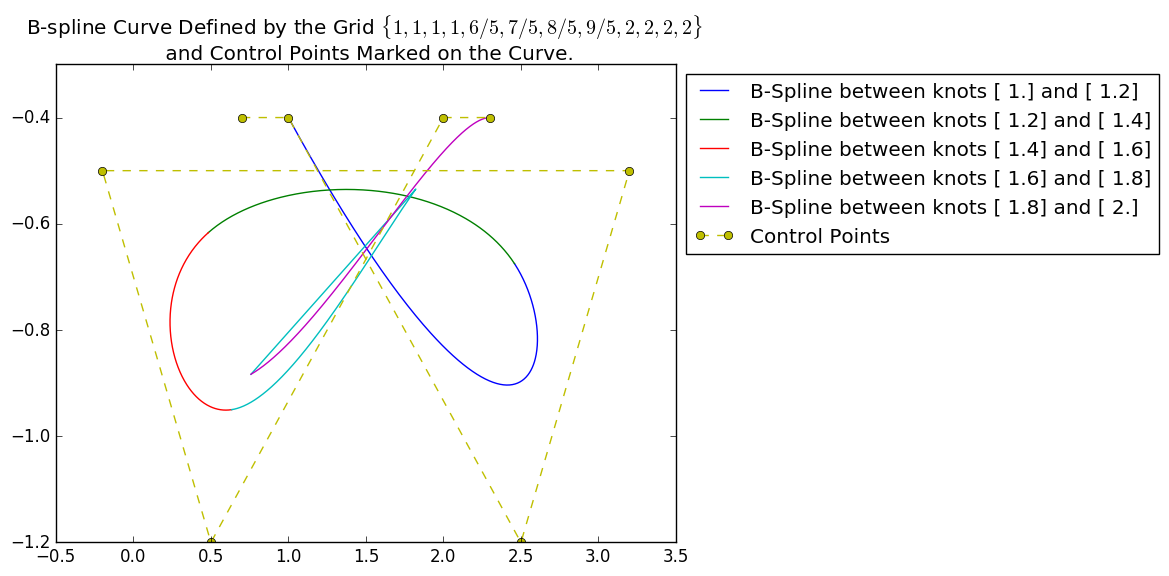
\includegraphics[scale=0.5]{task2}
\end{figure}

\section*{Task 3}
In this task we want to derive a relation between the number of control points $n+1$ of a clamped B-spline curve of degree $p$ and with simple knots, and the total number of control points of the curve's B\'{e}zier segments. We first determine the number of B\'{e}zier segments expressed in $n$ and then find the number of control points.
\subsection*{Number of B\'{e}zier segments}
In the case of only simple knots, including the endpoints, we know that the number of subintervals are given by \begin{equation}\label{subintervals}
\#\mathrm{subintervals} = \#\mathrm{knots} - 1.
\end{equation}
From \eqref{subintervals}, it is evident that in the present case, the number of B\'{e}zier segments is given by \begin{equation}\label{segments}
\#\mathrm{segments} = \#\mathrm{knots} - 2p - 1.
\end{equation}
Furthermore, we know that \begin{equation*}
\#\mathrm{knots} - 1 = \#\mathrm{controlpoints} + \mathrm{degree},
\end{equation*} 
or equivalently\begin{equation}\label{generalrelation}
\#\mathrm{knots} - 1 = n + 1 + p.
\end{equation}
Using \eqref{segments} and \eqref{generalrelation}, we have that \begin{equation}\label{segmentrelation}
\#\mathrm{segments} = n + 1 - p.
\end{equation}
\subsection*{Number of control points}
Every B\'{e}zier segments has the same degree $p$ as the original curve, resulting in every segment needing $p+1$ control points. As the inner control points are each used by two B\'{e}zier segments, one of the segment has $p+1$ unique control points, while the others have $p$ unique control points each. Using \eqref{segmentrelation}, we have that the total number of control points are given by\begin{equation*}
\begin{aligned}
\#\mathrm{total} &= p + 1 + p(n + 1 - p - 1)\\
&= p(n + 1 - p) + 1.
\end{aligned}
\end{equation*}
\subsection*{Comparison with control points of B-spline}
In the plot below, the relation of $n+1$ and the total number of control points of the B\'{e}zier segments can be seen. From \eqref{segmentrelation} we have that $n+1>p$, yielding the somewhat strange appearance of the plot. We see that the number of total number of control points of the B\'{e}zier segments is larger than the number of control points of the corresponding B-splines, except for the case $p=1$, where they are equal.

\section*{Task 4}
The B-spline curve is defined by the knots $\{0,0,0,0,0,1/3,2/3,1,1,1,1,1\}$ and the control points $(0,0)$, $(-4,0)$, $(-5,2)$, $(-4,4.5)$, $(-2,5)$, $(1,5.5)$ and $(1,0)$. By subdividing the curve at the points $1/3$ and $2/3$ we get three B\'{e}zier curves that represent the original B-Spline curve. The control points for the first B\'{e}zier segment are $(0,0)$, $(-1.3,0)$, $(-2.3,0.2)$, $(-3,0.6)$, $(-3.5,1.1)$, $(-3.7,1.6)$ and $(-3.7,2.1)$. For the second segment we have $(-3.7,2.1)$, $(-3.8,2.8)$, $(-3.4,3.5)$, $(-2.9,4.1)$, $(-2.1,4.4)$, $(-1.2,4.4)$ and $(-0.5,4)$. The third and last segment have the control points $(-0.5,3.7)$, $(-0.1,3.7)$, $(0.4,3.4)$, $(0.6,2.8)$, $(0.9,2.1)$, $(1,1.2)$ and $(1,0)$. The degree of each B\'{e}zier segment is determined by the number of control points of that segment minus one. Each segment has the same number of control points as the entire B-spline curve, hence the degree of each segment is $7-1=6$.

\begin{figure}[h!]
	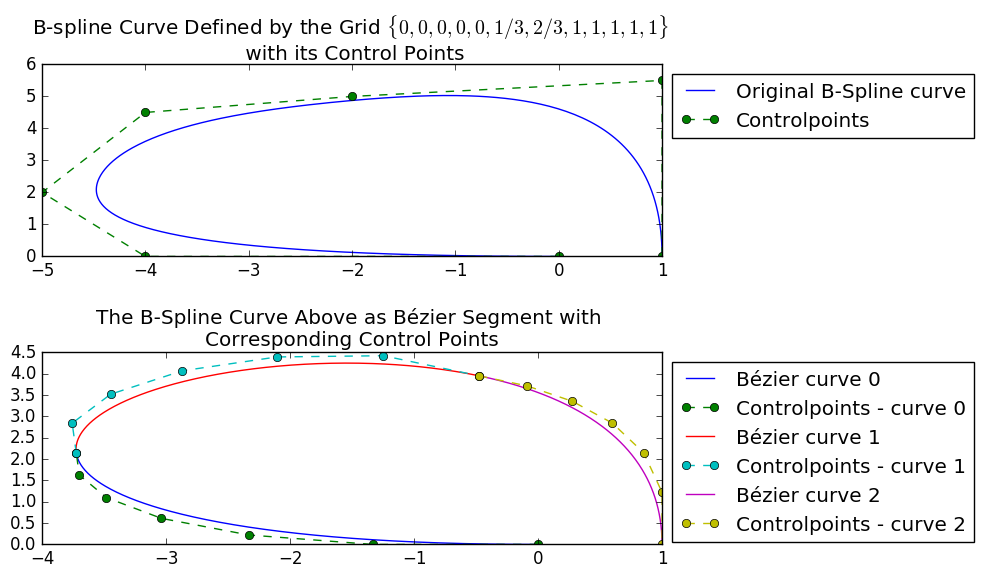
\includegraphics[scale=0.5]{task4}
\end{figure}

\section*{Task 5}
The curve constructed by the knots $$\{0,1/11,2/11,3/11,4/11,5/11,6/11,7/11,8/11,9/11,10/11,1\}$$ with control points $(0,0)$, $(3,2)$, $(9,-2)$, $(7,-5)$, $(1,-3)$, $(1,-1)$, $(3,1)$, $(9,-1)$ is shown in the first figure. The following figures show how the curve changes if we replace the last knot by the first one followed by the second last one with the second one and so on. 

What we can se from the pictures is that..

\begin{figure}[h!]
	%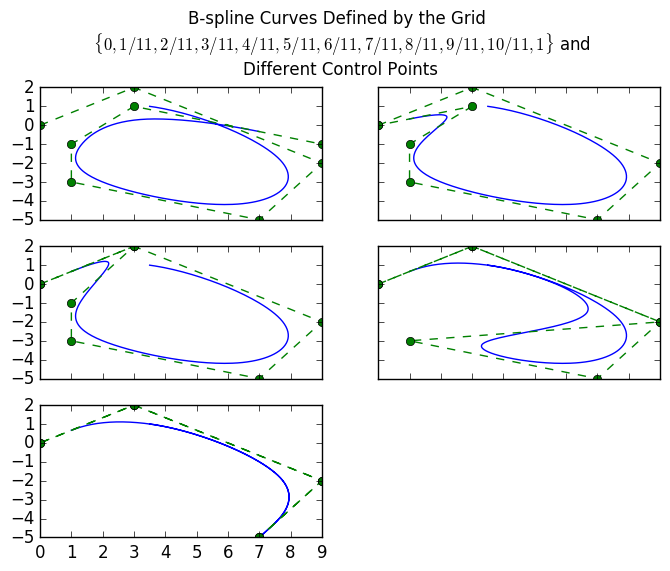
\includegraphics[scale=0.6]{task5}
\end{figure}


\section*{Task 6}
In this task we want to give a rational parametric representation of the segment of the unit circle in $\mathbb{R}^2$ for $x, y \leq 0$.\\
A natural parametrization of the circle is simply\begin{equation*}
\varphi(t) = \left(\begin{array}{c}
\sin(t)\\
\cos(t)
\end{array}\right).
\end{equation*}
We recall the Taylor expansions of sine and cosine\begin{equation}
\begin{aligned}
\sin(t) &= \sum_{k=0}^{\infty}(-1)^k\frac{t^{2k+1}}{(2k+1)!}\\
\cos(t) &= \sum_{k=0}^{\infty}(-1)^k\frac{t^{2k}}{(2k)!}
\end{aligned}
\end{equation}
$\forall t\in\mathbb{R}$. It is thus not possible to express the points on the circle as polynomials of finite degrees.\\
Consider the lines passing through the point (1, 0) and the segment of the unit circle with $x, y\leq 0$. All such lines are on the form \begin{equation}\label{lines}
y=t(x-1)\quad t\in[0, 1]\quad x\in[-1, 0].
\end{equation}
All points on the circle segment fulfills \begin{equation}\label{circle}
y^2 + x^2 = 1.
\end{equation} 
Now substitute $y$ in \eqref{circle} with $y$ in \eqref{lines}. This yields\begin{equation}\label{xequation}
x^2 + t^2(x - 1)^2 = 1.
\end{equation}
The solutions to \eqref{xequation} are given by $x=1$ and $x=\frac{t^2 - 1}{t^2 + 1}$ and since we need $x\in [-1, 0]$ only the second is suitable. Inserting this expression for $x$ into \eqref{circle} yields\begin{equation}\label{yequation}
y^2 + \left(\frac{t^2 - 1}{t^2 + 1}\right)^2 = 1.
\end{equation}
The solutions to \eqref{yequation} are given by $y=\frac{2t}{t^2 + 1}$ and $y=-\frac{2t}{t^2 + 1}$ and we are only interested in the second solution as $y\in[-1, 0]$.\\
Thus, the circle segment can be parametrized by \begin{equation*}
\varphi(t)=\frac{1}{t^2 + 1}\left(\begin{array}{c}
t^2 - 1\\
-2t
\end{array}\right).
\end{equation*}
A plot of the circle segment using the above parametrization can be seen below.
\begin{figure}[h!]
	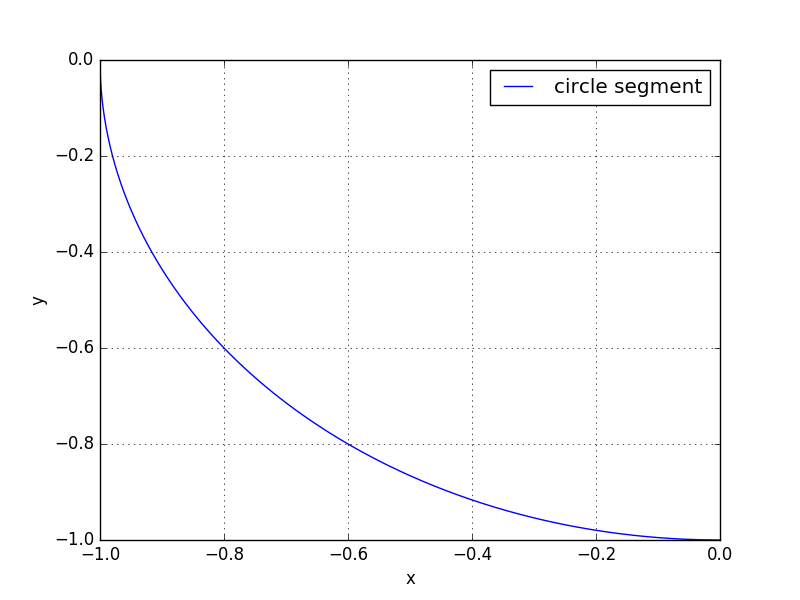
\includegraphics[scale=0.6]{circlesegment}
\end{figure}

\newpage
\section*{Appendix I}
\lstinputlisting{BsplineClass.py}

\end{document}
